\documentclass[runningheads]{llncs}

% Metadata Information
%\acmConference[DRAFT]{Draft paper}
%\acmJournal{PACMPL}
%\acmVolume{9}
%\acmNumber{4}
%\acmArticle{39}
%\acmYear{2010}
%\acmMonth{3}
%\copyrightyear{2009}
%\acmArticleSeq{9}

% Copyright
%\setcopyright{acmcopyright}
%\setcopyright{acmlicensed}
%\setcopyright{rightsretained}
%\setcopyright{usgov}
%\setcopyright{usgovmixed}
%\setcopyright{cagov}
%\setcopyright{cagovmixed}

% DOI
%\acmDOI{0000001.0000001}

% Paper history
%\received{February 2007}
%\received[revised]{March 2009}
%\received[accepted]{June 2009}

%\citestyle{acmauthoryear}

%%% PACKAGES %%%

\usepackage[inline]{enumitem}
\usepackage[nomargin,inline,draft]{fixme}
\usepackage{graphicx}
\usepackage{hyperref}
\usepackage{microtype}
\usepackage{pbox}
\usepackage{tikz}
\usepackage{url}
\usepackage{alltt}
%\usepackage[cache=false]{minted}
\usepackage{minted}
\usepackage{syntax}



% Must come after hyperref
\usepackage[capitalise]{cleveref}


%%% MINTED COMMANDS FOR HASKELL %%%

\newmint{haskell}{}
\newminted{haskell}{}
\newmintinline{haskell}{}

\FXRegisterAuthor{pls}{apls}{\color{teal}[Pablo]}
\FXRegisterAuthor{sjt}{asjt}{\color{magenta}[Simon]}

%%% MACROS %%%

\definecolor{myblue}{rgb}{0.2, 0.3, 1.0}
\newcommand{\bluett}[1]{\textcolor{myblue}{\texttt{#1}}}
\newenvironment{allbluett}{\begin{alltt}\color{myblue}}{\end{alltt}}
\newcommand{\ignore}[1]{} % for commenting out large portions, surround by \ignore{ and }

\setlength{\itemsep}{2pt}

% Document starts
\begin{document}


%
%
% Title portion. Note the short title for running heads
\title {Marlowe: financial contracts on blockchain\thanks{This work is part of the Cardano project 
and is supported by IOHK,~\url{https://iohk.io}}}
%
%\titlerunning{Abbreviated paper title}
% If the paper title is too long for the running head, you can set
% an abbreviated paper title here
%
\author{Pablo Lamela Seijas\orcidID{0000-0002-1730-1219}\\
\and Simon Thompson\orcidID{0000-0002-2350-301X}}
%
\authorrunning{P. Lamela Seijas and S. Thompson}
% First names are abbreviated in the running head.
% If there are more than two authors, 'et al.' is used.
%
\institute{School of Computing, University of Kent, Canterbury, UK}
\email{\{p.lamela-seijas,s.j.thompson\}@kent.ac.uk}


\begin{abstract}

Blockchains allow the specification of contracts in the form of programs that guarantee their fulfilment. 
Nevertheless, errors in those programs can cause important, and often irretrievable, monetary loss. General-purpose 
languages provide a platform on which contracts can be built, but by their very generality they have the potential to 
exhibit behaviours of an unpredictable kind, and are also not easy to read or comprehend for general users. 

An alternative solution is provided by domain-specific languages (DSLs), which are designed to express programs in a 
particular field. This paper explores the design of one DSL, Marlowe, targeted at the execution of financial 
contracts in the style of Peyton Jones \emph{et al} on blockchains. We present an executable semantics of Marlowe in 
Haskell, an example of Marlowe in practice, and describe the Meadow tool that allows users to interact in-browser with 
simulations of Marlowe contracts.

\end{abstract}


% The code below should be generated by the tool at
% http://dl.acm.org/ccs.cfm
% Please copy and paste the code instead of the example below.

%
% End generated code
%

\keywords{
  No keywords
}

\maketitle

% If the default list of authors is too long for headers, it can be redefined
%\renewcommand{\shortauthors}{}

\section{Introduction}
\label{sec:intro}


This paper explores the design of a domain specific language, Marlowe,\footnote{Named after Christopher 
Marlowe, the Elizabethan poet, dramatist and spy, who was born and educated in Canterbury,  
\url{en.wikipedia.org/wiki/Christopher_Marlowe}}\footnote{Marlowe is available from 
\url{https://github.com/input-output-hk/scdsl}} targeted at the execution of financial contracts in the style of 
Peyton Jones, Eber and Seward~\cite{PeytonJones:2000} on blockchains. In doing this, we are required to refine the 
model of contracts in a number of ways in order to fit with a radically different context. 

Consider the following example of an ``escrow'' contract so that we can explain the motivation 
more concretely. The aim of this contract, written in functional pseudocode in the style of~\cite{PeytonJones:2000} 
involves three participants: \haskellinline{alice}, \haskellinline{bob} and \haskellinline{carol}. \haskellinline{alice} 
is to pay an amount of money to \haskellinline{bob} on receipt of goods from her. \haskellinline{alice} pays the money 
into escrow controlled by \haskellinline{carol}.

There are two options for the money: if two out of the three participants agree to \haskellinline{pay} it to 
\haskellinline{bob}, that goes ahead; if, on the other hand, two of the participants opt to \haskellinline{refund} the 
money to \haskellinline{alice}, that is done instead.

The outer primitive \haskellinline{When} waits until the condition -- its first argument -- 
becomes true; in this case, the condition is that either two participants choose \haskellinline{refund} or two 
participants choose \haskellinline{pay}. The second argument of the \haskellinline{When} is itself another 
\haskellinline{Contract}, which is performed after the condition of the \haskellinline{When} has been met, and it makes 
the payment if two participants chose \haskellinline{pay}, otherwise it redeems previous money commitments.

\begin{haskellcode}
(When (Or (two_chose alice bob carol refund)
          (two_chose alice bob carol pay))
      (Choice (two_chose alice bob carol pay)
              (Pay alice bob AvailableMoney)
              redeem_original))
\end{haskellcode}

We discuss this particular example in more detail in Marlowe in Section~\ref{section:example-escrow} below; but it 
already gives us an example of how traditional contracts are fundamentally different from contracts that are meant to 
be run on top of the blockchain. In the traditional model, enforcement of the contract is the responsibility of the 
legal system. If \haskellinline{alice} does not pay the money into escrow, or \haskellinline{carol} chooses to keep it 
for herself, then they can be sued for the money (and probably damages), thus providing both legal and financial 
incentives for compliance. On the other hand, in the decentralised blockchain model, where there is no central 
authority, the contract needs to be enforced \emph{by design}.

This means that we must require participants to \emph{commit} money to cover all possible expenditure \emph{in advance 
of the contract executing}. In order to make sure that participants continue to engage with a contract, we ensure 
urgency by imposing \emph{timeouts}: money is committed for a finite period only. We also impose a timeout when waiting 
for a participant to make a commitment to ensure that the contract does not become stuck even if one of the participants 
stops interacting with it.

We make the following contributions in this paper.
\begin{itemize}
\item
Designing a DSL for financial contracts on blockchains: Marlowe.
\item
Defining an executable, small-step semantics of Marlowe in Haskell.
\item 
Making Marlowe an embedded DSL in Haskell. This extends the expressibility of the language, as we can use all the 
facilities of Haskell in defining Marlowe contracts; we achieve this by defining Marlowe as  a Haskell 
\haskellinline{data} type.
\item
Developing the Meadow tool that allows users to interact with and simulate the operation of Marlowe contracts 
and embedded Marlowe contracts.
\end{itemize}

Having established this model and its semantics we are able to do a number of other things, which we discuss in the 
paper. We can explore how the language will be implemented on an existing blockchain, such as Cardano, and our model has 
shown us that we will need to consider how the evolution of a contract interacts with the blockchain, with miners in the 
case of a `proof of work'-based chain, and with users participating in contract execution. We can also perform analyses 
of Marlowe contracts, based on its formal semantics. 

In designing a language like Marlowe we are constrained by the blockchain domain, but within that we do have a range of 
choices. For example, should we base the language on a system with accounts, like Ethereum, or a UTxO-based model as 
used by bitcoin? We examine this and other choices after introducing the language and examples of its use. 


%Moreover, there is not a single blockchain model, and we give a brief overview of the different mechanisms for 
%scripting on blockchain (although this is not the primary purpose of this article). 
%A particularly important technical distinction here is that between an account-style model as used by 
%Ethereum~\cite{EthereumRationale}, and the unspent transaction output (UTxO) model of bitcoin~\cite{sok}. 
%There is also the question of how precisely the execution of the contract interacts with the blockchain, and how 
%information is to be recorded on the chain. Finally, should the execution ``push'' for changes  to happen, or do 
%external actors have to ``pull'' to effect changes enabled by execution of the contract?
%
%The paper describes version 1.3 of Marlowe, and it should be seen as a work in progress. We have designed it to provide 
%financial contracts in Cardano, but also in order to start to answer the twin questions of what smart contracts will 
%look like in Cardano, and how those contracts will be implemented in the overall system.
 
The paper begins in Section \ref{section:model} by introducing the Marlowe 
model, including the assumptions made in designing it, the types of the principal functions and a description of the 
DSL as an algebraic type, constructor by constructor. 
%Section \ref{section:example-saving} presents an example of a larger Marlowe contract, for incentivised saving. 
Section \ref{section:example-escrow} revisits the escrow example, and shows 
how it is described using a combination of Marlowe and Haskell constructs: that is, we use Marlowe as an embedded DSL. 
Section \ref{section:tool} introduces Meadow, our tool for visualising and interacting with Marlowe contracts.
Section \ref{sec:abstraction} reflects on the design rationale for Marlowe, showing how it can be supported on a variety of 
blockchains, and Section \ref{sec:compilation} explores how Marlowe can be implemented. Section \ref{sec:related} 
surveys related work and Section 
\ref{section:next-steps} enumerates the next steps for the project after drawing some conclusions.

\begin{figure}[t]
\begin{center}
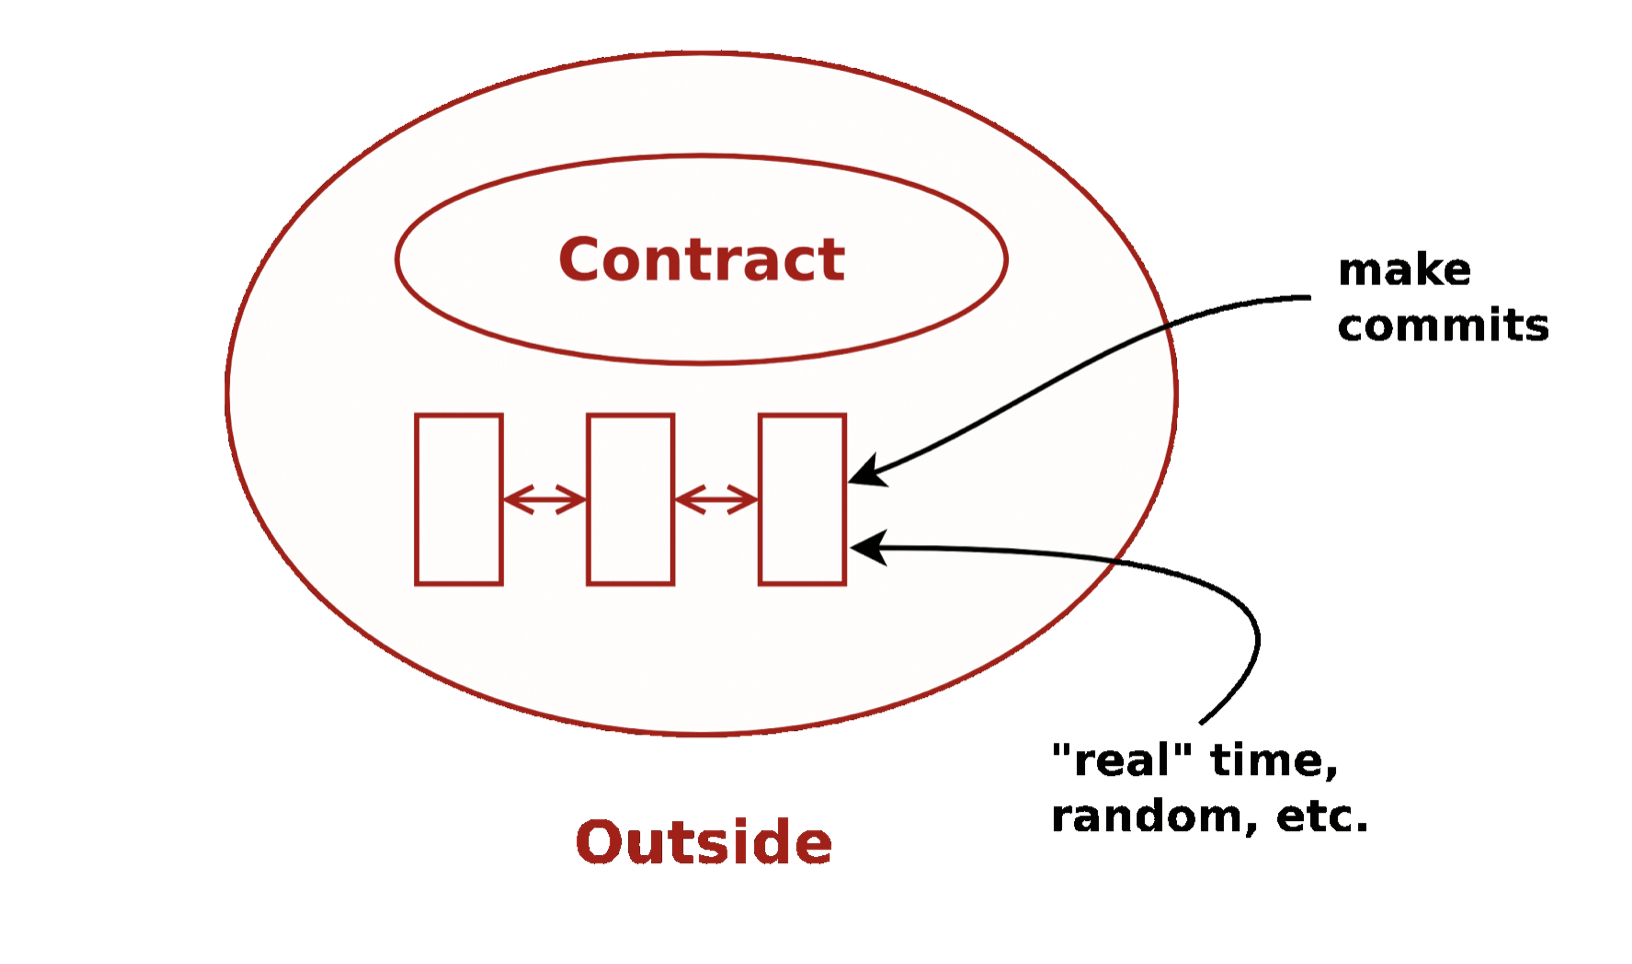
\includegraphics[width=0.6\textwidth]{pix/context.png}
\caption{The context for a contract}
\label{fig:context}
\end{center}
\vspace*{-8mm}
\end{figure}


\section{The Marlowe model}
\label{section:model}

The Marlowe domain-specific language (DSL) is modelled as an algebraic type in Haskell, together with an executable 
small-step semantics. We start by looking at the different types used by the model, and the assumptions about the 
infrastructure in which contracts will be run. We then we look at the \haskellinline{Contract} DSL itself, 
and finally we give its semantics in Haskell. Section 
%\ref{section:example-saving} gives an example of Marlowe in action, and Section
\ref{section:example-escrow} revisits the ``escrow'' example using the embedding of Marlowe as a DSL in Haskell.

\subsection{The model types}

A running contract interacts with its environment in two ways, as in Figure \ref{fig:context}.

\paragraph{Observables}


First, it will need to observe different kinds of varying quantities including, for example, the current time, the 
current block number and, random numbers, as well as ``real world'' quantities like ``the price of oil'' or ``the 
exchange rate between currencies A and B''. 
As the examples illustrate, observables come both from aspects of the blockchain (e.g.\ the current block number) and 
externally. In the latter case, it will be necessary to agree a trusted oracle or beacon giving the value.


Each instance of such an observable will be observed at a particular time and in a particular context. We assume that 
the system infrastructure ensures that these values are recorded on the blockchain to allow the computation to be 
repeated for verification purposes. 


It is assumed that at each step of the execution of the contract, the values of observables will be available if 
needed, and these values are (together) given by a value of type \haskellinline{OS} (for ``observable set''), where 
individual observations are described in a ``little language'' for that purpose: \haskellinline{Observation}. 
Note that these values are not determined by the participants in the contract, but rather by the external environment in 
which the contract is run.

 

\paragraph{Inputs and Commitments}


On the other hand, at each step there are -- potentially, at least -- a variety of inputs available from the 
participants themselves. These include commitments of currency (or ``cash''), redemption of commitments, and claims of 
payments by a participant. Moreover, it is also possible for a participant to input an arbitrary value (which we term a 
``choice''). The particular inputs at a given step are described by a value of type \haskellinline{Input}.

%\paragraph{Commitments}


While informally we might see a commitment to something as being indefinite, it is important to realise that, 
on blockchain, a commitment needs to have a timeout so that progress can be forced in a contract. After the timeout 
period the cash can be refunded through the user creating a transaction to reclaim the cash. Information about the 
commitments currently in force forms the \haskellinline{State}, which can be  modified at each execution step. 

\paragraph{Actions}

Payments can be granted by using committed money, but they must be manually redeemed by the recipient, in the 
same way that cash commitments are redeemed when they expire. The effects of the contract in the blockchain are 
represented by a list \haskellinline{AS} of \haskellinline{Actions} that is derived from the execution of each step of 
the semantics.

\begin{figure}[t]
\begin{center}
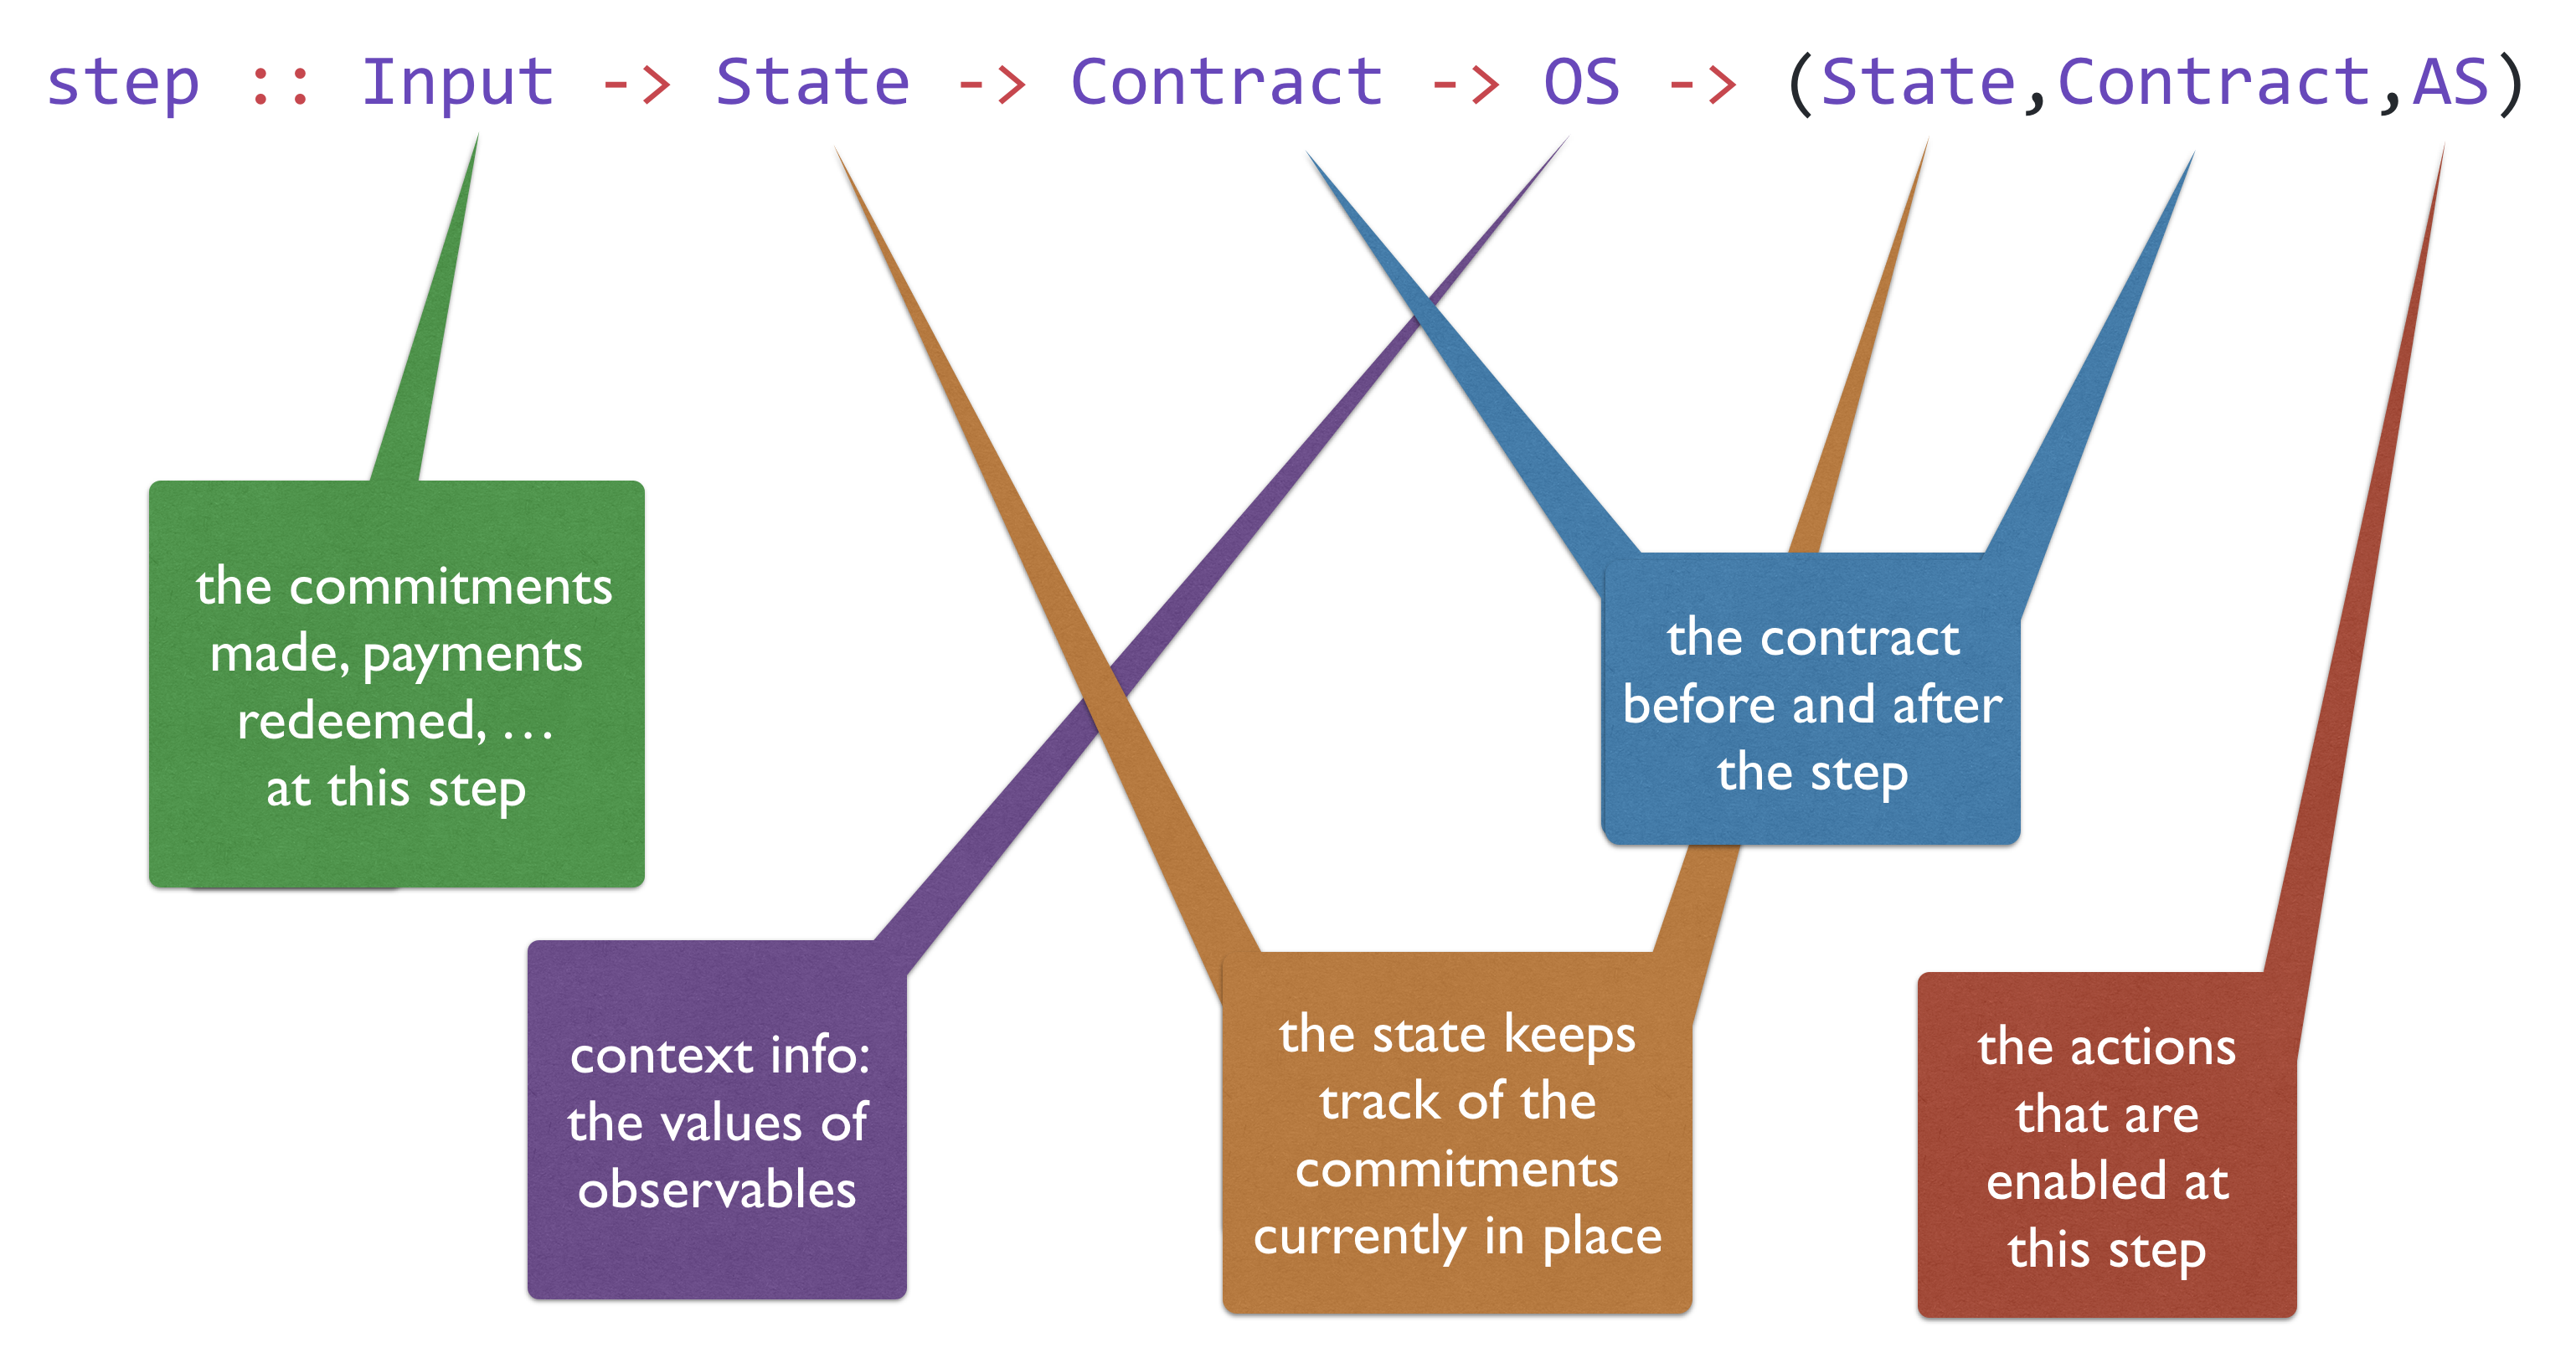
\includegraphics[width=0.8\textwidth]{pix/step-type.png}
\caption{The \haskellinline{step} function}
\label{fig:step-function}
\end{center}
\vspace*{-8mm}
\end{figure}

\paragraph{Infrastructure}

The model makes a number of assumptions about the blockchain infrastructure in which it is run.

\begin{itemize}
\item It is assumed that cryptographic functions and operations are provided by a layer external to the system, and so 
they need not be modelled explicitly.
\item We assume that time is ``coarse grained'' and measured by block number, so that, in particular, timeouts are 
delimited using block numbers. 
\item 
Making a commitment is not something that a contract can perform; rather, it 
can request that a commitment is made, but that then has to be established externally: hence the input of (a set of) 
commitments at each step.
\item The model manages the release of funds back to the committer when a cash commitment expires (see discussion of 
the \haskellinline{stepBlock} function below).
\end{itemize}

\paragraph{Computation}

Computation is modelled at two different levels. 

The \haskellinline{step} function represents a \emph{single computation step} and has this type:
\begin{haskellcode}
step :: Input -> State -> Contract -> OS -> (State,Contract,AS)
\end{haskellcode}
which is also illustrated in Figure \ref{fig:step-function}. 
The \haskellinline{step} function is total, so that for every contract a result of stepping is defined. However, for 
some kinds of contracts -- commits, redeems or time-shifted contracts -- it is possible that performing  a step 
produces the same contract as the result; we call these \emph{quiescent} steps whereas all others \emph{make 
progress}. We use this distinction in the explanation that follows.

Execution of a contract will involve multiple blocks, with multiple steps in each block. The computation at a single 
block is given by the \haskellinline{stepBlock} function: this will call the \haskellinline{stepAll} function that calls 
\haskellinline{step} repeatedly until it is quiescent. 

In addition to calling \haskellinline{stepAll}, \haskellinline{stepBlock} will first enable expired cash commitments to 
be refunded and record, in the state, any choices made at that step. The functions \haskellinline{stepAll} and 
\haskellinline{stepBlock} have the same type as \haskellinline{step} itself.





\subsection{The \haskellinline{Contract} type}

The type of contracts is given by the following Haskell data type:

\begin{haskellcode}
data Contract =
   Null |
   CommitCash IdentCC Person Money Timeout Timeout Contract Contract |  
   RedeemCC IdentCC Contract |
   Pay IdentPay Person Person Money Timeout Contract |  
   Both Contract Contract |
   Choice Observation Contract Contract |
   When Observation Timeout Contract Contract   
   \end{haskellcode}
Informally, this type provides a \haskellinline{Null} contract, which does nothing. The next three constructs form 
contracts that do something, and then continue according to another contract (which is one of the components of the 
original contract). \haskellinline{CommitCash} will wait for a participant to make a commitment, 
\haskellinline{RedeemCC} allows for a commitment to be redeemed, and \haskellinline{Pay} for a payment between 
participants to be claimed by the recipient. 

The remaining constructors form composite contracts from simpler components: \haskellinline{Both} has the behaviour of 
both its components, \haskellinline{Choice} chooses between two contracts on the basis of an observation, and 
\haskellinline{When} is quiescent until a condition -- i.e.\ an \haskellinline{Observation} -- becomes true.

Additionally, many of the contracts have timeouts that also determine their behaviour. 
\subsection{The \haskellinline{step} function}

In this section, we explain the detailed behaviour of contracts by describing how the \haskellinline{step} function 
operates on each of the constructors of the \haskellinline{Contract}  type.

\begin{itemize}
\item \haskellinline{Null} is the null contract; it will always be quiescent:

\begin{haskellcode}
step _ st Null _ = (st, Null, [])
\end{haskellcode}

\medskip
\noindent
\item \haskellinline{CommitCash ident person val start_timeout end_timeout con1 con2}  For this contract to make 
progress,\begin{itemize}
\item either, before the timeout \haskellinline{start_timeout}, the user \haskellinline{person} makes a cash commitment 
of value 
\haskellinline{val} and timeout \haskellinline{end_timeout}  with the identifier \haskellinline{ident}, 
\item
or the timeout \haskellinline{start_timeout} is exceed:
\end{itemize} 

\begin{haskellcode}
step 
  commits 
  st 
  c@(CommitCash ident person val start_timeout end_timeout con1 con2) 
  os
  | cexe || cexs = (st {sc = ust}, con2, [])
  | Set.member (CC ident person cval end_timeout) (cc commits)
        = (st {sc = ust}, con1, [SuccessfulCommit ident person cval])
  | otherwise = (st, c, [])
  where ccs = sc st
        cexs = expired (blockNumber os) start_timeout
        cexe = expired (blockNumber os) end_timeout
        cns = (person, if cexe || cexs 
                          then ManuallyRedeemed 
                          else NotRedeemed cval end_timeout)
        ust = Map.insert ident cns ccs
        cval = evalMoney st val
\end{haskellcode}
In the first case, a \haskellinline{SuccessfulCommit} action is generated and the contract continues as 
\haskellinline{con1}; in the second case no action is generated and the contract continues as 
\haskellinline{con2}. While neither case holds, the contract is quiescent, waiting for the cash to be committed. 

If the cash is committed successfully and the timeout \haskellinline{end_timeout} is reached, then it is impossible to 
further spend the committed cash, and any unspent funds can be reclaimed by \haskellinline{person}.
 This is enforced by the \haskellinline{stepBlock} function, as noted above.

\medskip
\noindent
\item \haskellinline{RedeemCC ident con} (\haskellinline{CC} stands for cash commitment.) For this contract to make 
progress, the creator of the cash commitment with identifier \haskellinline{ident} is allowed to redeem the unspent 
funds in that commitment; the contract then continues as \haskellinline{con}, and the action 
\haskellinline{CommitRedeemed} is produced. 

\begin{haskellcode}
step commits st c@(RedeemCC ident con) _ =
    case Map.lookup ident ccs of
      Just (person, NotRedeemed val _) ->
        let newstate = 
                st {sc = Map.insert ident (person, ManuallyRedeemed) ccs} in
        if Set.member (RC ident person val) (rc commits)
        then (newstate, con, [CommitRedeemed ident person val])
        else (st, c, [])
      Just (person, ManuallyRedeemed) ->
        (st, con, [DuplicateRedeem ident person])
      Nothing -> (st,c,[])
    where
        ccs = sc st
\end{haskellcode}
Committed cash can only be redeemed once, and an attempt to redeem it a second time will produce a  
\haskellinline{DuplicateRedeem} action, continuing as \haskellinline{con}.

If the cash commitment with identifier \haskellinline{ident} has expired, it becomes possible for the remaining funds 
to be redeemed by the committer; this can be done by the \haskellinline{stepBlock} function processing the appropriate 
\haskellinline{Input}, and an \haskellinline{ExpiredCommitRedeemed} action will be produced. 

Once the commitment \haskellinline{ident} has expired and is redeemed, a \haskellinline{RedeemCC ident con} contract 
will 
immediately evolve to \haskellinline{con}.
%\footnote{How does the contract determine what actions resulted from a given step? Or is this not required?}
%\footnote{If it is required, restructuring the DSL so that the result action appears as the 'value' of executing a 
%          step (using a monadic interface as described for id generation below) would be a good idea.}
%\footnote{We specify the actions generated by each kind of constructor; at each step the list of such actions, of type 
%          \haskellinline{AS}, is a component of the result.}. 

\medskip
\noindent
\item \haskellinline{Pay idpay from to val expi con} makes it possible, assuming that sufficient funds are available, 
for \haskellinline{to} to claim a payment with id \haskellinline{idpay} of \haskellinline{val} from 
\haskellinline{from} before the timeout \haskellinline{expi}. The contract continues as \haskellinline{con}. 

\begin{haskellcode}
step inp st c@(Pay idpay from to val expi con) os
  | expired (blockNumber os) expi = (st, con, [ExpiredPay idpay from to cval])
  | right_claim =
    if ((committed st from bn >= cval) && (cval >= 0))
      then (newstate, con, [SuccessfulPay idpay from to cval])
      else (st, con, [FailedPay idpay from to cval])
  | otherwise = (st, c, [])
  where
    cval = evalMoney st val
    newstate = stateUpdate st from to bn cval
    bn = blockNumber os
    right_claim =
      case Map.lookup (idpay, to) (rp inp) of
        Just claimed_val -> claimed_val == cval
        Nothing -> False
\end{haskellcode}
By `available' we mean that sufficient commitments have been made and not yet expired to cover the payment; in this 
case, the payment uses the currency allocated by the cash commitments made by \haskellinline{from} that expire the 
earliest.

This contract will result in a \haskellinline{FailedPay} action if the funds are not available; otherwise a 
\haskellinline{SuccessfulPay} action is generated.

\medskip
\noindent
\item \haskellinline{Both con1 con2} enforces the behaviour of both contracts \haskellinline{con1} and 
\haskellinline{con2}. 
\begin{haskellcode}
step comms st (Both con1 con2) os =
    (st2, result, ac1 ++ ac2)
    where
        result | res1 == Null = res2
               | res2 == Null = res1
               | otherwise = Both res1 res2
        (st1,res1,ac1) = step comms st con1 os
        (st2,res2,ac2) = step comms st1 con2 os
\end{haskellcode}
Because the model is stateful and produces output actions, to make a step, it is necessary to execute a single step of 
each of  the contracts \haskellinline{con1} and \haskellinline{con2} in sequence: first \haskellinline{con1} then 
\haskellinline{con2}.

\medskip
\noindent
\item \haskellinline{Choice obs conT conF} behaves as either \haskellinline{conT} or \haskellinline{conF} depending on 
the 
(Boolean) result of \haskellinline{obs} at the time that the observation is made, \haskellinline{conT} if it is 
\haskellinline{True} and \haskellinline{conF} if \haskellinline{False}.

\begin{haskellcode}
step _ st (Choice obs conT conF) os =
    if interpretObs st obs os
        then (st,conT,[])
        else (st,conF,[])
\end{haskellcode}

\medskip
\noindent
\item \haskellinline{When obs expi con con2} This contract will not progress until \haskellinline{obs} is 
\haskellinline{True} or until the current block number is greater than or equal to the one specified by timeout 
\haskellinline{expi}. In case the timeout applies, the contract will continue as \haskellinline{con2}, if the timeout 
does not apply and \haskellinline{obs} is \haskellinline{True}, then the contract continues as \haskellinline{con}. 
Otherwise the contract is quiescent.

\begin{haskellcode}
step _ st (When obs expi con con2) os
  | expired (blockNumber os) expi = (st,con2,[])
  | interpretObs st obs os = (st,con,[])
  | otherwise = (st, When obs expi con con2, [])
  \end{haskellcode}
\end{itemize}
We look next at an example of Marlowe in action.


\ignore{ % begin ignore

\section{Incentivised saving}
\label{section:example-saving}

In this section, we show how Marlowe can be used for designing a contract that incentivises saving. We use the 
following example: \haskellinline{bob} offers 20 ADA to \haskellinline{alice} in exchange for saving 100 ADA for 100 
blocks. \haskellinline{alice} will be able to withdraw the savings after block 20, but if that option is chosen, then 
\haskellinline{bob} will not pay the extra 20 ADA to \haskellinline{alice}.

We will start from outer to inner primitives. The first thing is to allow \haskellinline{alice} to commit the 
100 ADA. The primitive says that with identity \haskellinline{IdentCC 1} (this is the identity of the commitment), 
\haskellinline{alice} can commit \haskellinline{100} ADA before block \haskellinline{10}, and the commitment 
must expire on block \haskellinline{200}. But if the money is not committed before block \haskellinline{10}, then the 
contract will continue as \haskellinline{Null}.

\begin{haskellcode}
CommitCash (IdentCC 1) 1 (ConstMoney 100) 10 200
           step2
           Null
\end{haskellcode}

If the commitment is done correctly and on time, we continue as in \haskellinline{step2}. \haskellinline{step2} is 
another commitment, this time by \haskellinline{bob}. The primitive says that with identity 
\haskellinline{IdentCC 2}, \haskellinline{bob} can commit \haskellinline{20} ADA before block 
\haskellinline{20}, and the commitment must expire on block \haskellinline{200}. But if the money is not committed 
before block \haskellinline{20}, then the contract will continue as \haskellinline{RedeemCC (IdentCC 1) Null}, which in 
turn gives \haskellinline{alice} the opportunity to withdraw all the money committed immediately.

\begin{haskellcode}
CommitCash (IdentCC 2) 2 (ConstMoney 20) 20 200
           step3
           (RedeemCC (IdentCC 1) Null)
\end{haskellcode}

If the commitment is done correctly and on time, we continue as in \haskellinline{step3}. \haskellinline{step3}
waits until choice with identity \haskellinline{IdentChoice 1} is made by \haskellinline{alice} or
until block \haskellinline{100} (whatever happens first). If the choice is made before block \haskellinline{100}, 
it continues as \haskellinline{stepRedeem}, if block \haskellinline{100} comes first, then it continues as 
\haskellinline{step4}.

\begin{haskellcode}
When (PersonChoseSomething (IdentChoice 1) 1) 100
     stepRedeem
     step4
\end{haskellcode}

\haskellinline{step4} pays the \haskellinline{20} ADA committed by \haskellinline{bob} in the commit with 
identity \haskellinline{IdentPay 1} to \haskellinline{alice}, if the payment is claimed before block 
\haskellinline{200}. Once the payment is claimed or after block 200, it continues as \haskellinline{stepRedeem}.

\begin{haskellcode}
Pay (IdentPay 1) 2 1 (ConstMoney 20) 200 stepRedeem
\end{haskellcode}

Finally, \haskellinline{stepRedeem} allows both participants to redeem all the remaining committed funds.

\begin{haskellcode}
Both (RedeemCC (IdentCC 1) Null)
     (RedeemCC (IdentCC 2) Null)
\end{haskellcode}

The whole contract remains as follows:
\begin{haskellcode}
CommitCash (IdentCC 1) 1
           (ConstMoney 100)
           10 200
           (CommitCash (IdentCC 2) 2
                       (ConstMoney 20)
                       20 200
                       (When (PersonChoseSomething (IdentChoice 1) 1)
                             100
                             (Both (RedeemCC (IdentCC 1) Null)
                                   (RedeemCC (IdentCC 2) Null))
                             (Pay (IdentPay 1) 2 1
                                  (ConstMoney 20)
                                  200
                                  (Both (RedeemCC (IdentCC 1) Null)
                                        (RedeemCC (IdentCC 2) Null))))
                       (RedeemCC (IdentCC 1) Null))
           Null
\end{haskellcode}

In the next section, we look at how to take advantage of Haskell embedding when implementing Marlowe contracts.


} % end ignore

\section{Marlowe as an embedded DSL}
\label{section:example-escrow}

In this section, we revisit the escrow example that we discussed briefly in the introduction, and show how we can make 
Marlowe contracts that are easier to write, read, and understand, by embedding them into Haskell code, that is, taking 
advantage of the fact that Marlowe contracts are implemented as Haskell terms to write Haskell programs that generate 
Marlowe code, instead of writing Marlowe directly.

We used Haskell because it is the language in which Marlowe is implemented, but it would be easy to embed Marlowe in any 
other language. It would only be necessary to translate its primitives into a data type in that language. In Meadow we 
use Fay \cite{Fay}, a subset of Haskell that we discuss in more detail in Section~\ref{section:tool}).

The example we use through this section implements an escrow contract, as first introduced in Section~\ref{sec:intro}. 
%
%Let us imagine that participant 
%\haskellinline{alice} is buying some item from \haskellinline{bob}. On one hand, if \haskellinline{alice} 
%pays before receiving the item, there is a risk that \haskellinline{bob} will never give \haskellinline{alice} the 
%item. On the other hand, if \haskellinline{bob} gives \haskellinline{alice} the item before 
%\haskellinline{alice} pays,  there is a risk that \haskellinline{alice} will never pay.
%
The escrow mechanism allows \haskellinline{alice} to deposit the money into a contract, in a way that the 
money will only be released when two out of three participants agree on whether \haskellinline{bob} has indeed 
given \haskellinline{alice} the item. 

The escrow participant (\haskellinline{carol}) is supposed to be a neutral third party that will decide in case of 
dispute. This way, if participants \haskellinline{alice} and \haskellinline{bob} are honest, they will just agree on 
the result of the transaction and \haskellinline{carol} will not need to do anything. If \haskellinline{alice} and 
\haskellinline{bob} disagree, \haskellinline{carol} will be able to choose whether the money must go to 
\haskellinline{alice} or to \haskellinline{bob}.

In our implementation we make things more specific: the money paid for the item is 450 ADA, and it must be committed by 
\haskellinline{alice} before block \haskellinline{10}; it will be refunded to \haskellinline{alice} if 
there is no consensus before block \haskellinline{90}.

We start by defining some Haskell functions. We can encapsulate identifiers in functions to make the contract more 
readable. That way we can generate an identifier for the cash commitment:

\begin{haskellcode}
iCC1 :: IdentCC
iCC1 = IdentCC 1
\end{haskellcode}
An identifier for the payment:
\begin{haskellcode}
iP1 :: IdentPay
iP1 = IdentPay 1
\end{haskellcode}
And we can create identifiers for all the participants:
\begin{haskellcode}
alice, bob, carol :: Person
alice = 1
bob   = 2
carol = 3
\end{haskellcode}
We can also create a sub-contract that allows the money from the commitment with identifier \haskellinline{IdentCC 1} 
to be redeemed:
\begin{haskellcode}
redeem_original :: Contract
redeem_original = RedeemCC iCC1 Null
\end{haskellcode}
Once redeemed, the contract continues as \haskellinline{Null} since we expect this to be the last thing that is done.
Each participant has a say on who deserves the money: either \haskellinline{alice} deserves a refund, which 
we represent with the number $0$; or \haskellinline{bob} deserves a payment, which we represent with the 
number $1$. Because there is only one choice to make per participant, we use the same \haskellinline{IdentChoice} as 
their participant id. We can define a function that returns an observation that is true if and only if
\haskellinline{per} has chosen the number \haskellinline{c} for the choice \haskellinline{IdentChoice per} as follows:
\begin{haskellcode}
chose :: Int -> ConcreteChoice -> Observation
chose per c = PersonChoseThis (IdentChoice per) per c
\end{haskellcode}
Then, we can easily write a function that returns an observation that is \haskellinline{True} if and only if at least 
one of the participants \haskellinline{per} and \haskellinline{per'} has chosen the number \haskellinline{val} as 
follows:
\begin{haskellcode}
one_chose :: Person -> Person -> ConcreteChoice -> Observation
one_chose per per' val = (OrObs (chose per val) (chose per' val)) 
\end{haskellcode}
Building on that, we can now write a function that returns an observation that is \haskellinline{True} if and only if 
at least two out of the three participants \haskellinline{p1}, \haskellinline{p2}, and \haskellinline{p3} have agreed 
in choosing the number \haskellinline{c} as follows:
\begin{haskellcode}
two_chose :: Person -> Person -> Person -> ConcreteChoice -> Observation
two_chose p1 p2 p3 c = OrObs (AndObs (chose p1 c) (one_chose p2 p3 c))
                             (AndObs (chose p2 c) (chose p3 c))
\end{haskellcode}
Finally, we can write the escrow contract, thus:
\begin{haskellcode}
escrow :: Contract
escrow = CommitCash iCC1 1 (ConstMoney 450) 10 100
                    (When (OrObs (two_chose alice bob carol 0)
                                 (two_chose alice bob carol 1))
                          90
                          (Choice (two_chose alice bob carol 1)
                                  (Pay iP1 alice bob (AvailableMoney iCC1) 100
                                       redeem_original)
                                  redeem_original)
                          redeem_original)
                    Null
\end{haskellcode}

The outermost primitive \haskellinline{CommitCash} allows the \haskellinline{alice} to commit 
\haskellinline{450} ADA before block \haskellinline{10}, with the promise that money will be released on block 
\haskellinline{100} if they are not claimed before that.

The next primitive, \haskellinline{When}, waits for one of three things to happen:
\begin{enumerate}
	\item The observation became \haskellinline{True} because two out of three have chosen \haskellinline{0}. 
	\item The observation became \haskellinline{True} because two out of three have chosen \haskellinline{1}.
	\item The observation remained \haskellinline{False} until \haskellinline{90} was published in the blockchain.
\end{enumerate}

If the third option happens, the money is refunded. Otherwise, there is a \haskellinline{Choice} that will 
immediately refund the money to \haskellinline{alice} unless two out of three chose option 
\haskellinline{1}; 
in the later case, \haskellinline{Pay} will give \haskellinline{bob} the opportunity to claim the funds 
available in the commitment with identifier \haskellinline{iCC1} before block \haskellinline{100} (by using the 
identifier \haskellinline{iP1} for the claim). If the funds are not claimed before block \haskellinline{100} they will 
also be refunded to \haskellinline{alice}.

Reflecting on the example, we can see that using Haskell definitions has made the contract substantially more 
comprehensible. While our current implementation does not do this, it is possible to modify the embedding to support 
more efficient operation, by preserving \emph{sharing} in the host language. For example, if we were to replace the 
repeated  expression 
\haskellinline{two_chose alice bob carol 1} by a \haskellinline{where} clause, 
\begin{haskellcode}
escrow = ...        (When (OrObs (two_chose alice bob carol 0)
                                 chose_refund)
                          90
                          (Choice chose_refund ...
                           ...
         where chose_refund = two_chose alice bob carol 1                 
\end{haskellcode}
then the repeated computation of the expression could be avoided.
%In the next section, we cover the online contract visualisation and interaction tool for Marlowe.

\section{Visualising and interacting with Marlowe contracts}

\label{section:tool}

For Marlowe to be usable in practice, users need to be able to understand how contracts will behave once deployed to 
the blockchain, but without doing the deployment. We can do that by simulating their behaviour off-chain, interactively 
stepping through the evaluation of a contract in a browser. We do this in two stages, first transforming an embedded 
contract (using features of Haskell) to a pure Marlowe contract, and then interactively stepping through that contract.

To achieve this, and to aid Marlowe's take-up
usage by people that does not know or are not familiar with its syntax,
we have developed Meadow, a web tool that supports the interactive construction,
revision, and simulation of smart-contracts written in Marlowe. The
tool is publicly available in the url: \url{https://input-output-hk.github.io/scdsl/}.
In Figure~\ref{fig:full-screenshot-demo}, we provide a screenshot
of Meadow in the middle of simulating the execution of the ``deposit incentive'' contract available
in the GitHub repository (in the file: \texttt{src/DepositIncentive.hs}) and in the examples section of Meadow (on the 
bottom right part).

Meadow has been mainly written in Haskell and compiled to JavaScript
partially by the Haste compiler~\cite{Haste} and partially by GHCJS \cite{GHCJS};
Meadow also relies on the Blockly library~\cite{Blockly} for providing a visual
editor for smart contracts written in Marlowe. Embedding support in Meadow
is provided through a pruned and bundled version of the Fay compiler \cite{Fay},
compiled to JavaScript using GHCJS. All text fields that edit and present Meadow and Fay code are
instances of CodeMirror text editor \cite{CodeMirror}.

Blockly's editor allows the user to visualise and edit
smart-contracts as interlocking blocks that can be dragged and dropped
like pieces of a jigsaw puzzle. % (see Figure~\ref{fig:detail-of-block}).
Meadow also provides functionality to generate syntactically correct
and formatted code (that is displayed in the upper right corner of the application),
and to convert the code back to its Blockly representation.

Additionally, Meadow allows the user to use Meadow's Fay embedding from within the browser. % (see Figure~\ref{fig:embedded-demo}). 

The reason that we chose Fay instead of Haskell for Meadow is a technical one: we wanted Meadow to be run completely inside 
the browser, because that makes it easy to deploy, since the server is only required to send the page and not to 
run any Marlowe-related computation. There exist compilers from Haskell to JavaScript but most of them are not easy to 
bootstrap into JavaScript. Among other reasons, they often rely on the API of the host OS to read and write files.

The Fay compiler, on the other hand, is mostly written in pure Haskell, and it is not hard to compile to JavaScript by 
using GHCJS. Nevertheless, it does not include a type checker, it relies in GHC's type-checker; and it also 
tries to read its \haskellinline{Prelude} from disk. We have worked around these issues by disabling type-checking 
within Meadow embedded editor, and by embedding all the required modules as constant strings in a modified version 
of the Fay compiler.

In particular, Meadow includes a pruned copy of the Fay compiler, bundled with its Prelude module, its foreign 
interface, and a module with the definitions of the Marlowe primitives and a function to pretty-print 
Marlowe contracts. This allows the user to compile and execute, inside Meadow, Fay code that generates and prints 
a Marlowe contract. When the user opens the embedded editor, the current Marlowe contract is embedded into a template 
of a Fay program that prints it. The user is able to modify this code in the left panel of the editor and use the 
advanced functionalities provided by Fay like, for example, bindings, list-comprehensions, turing-complete functions 
definitions, etc.

When the user clicks the execute button, the Fay code is compiled to JavaScript and evaluated; this causes the Marlowe 
contract generated by the execution of the code to be written to the panel on the right. Generated contracts can then be 
sent back to the main screen of Meadow, translated to Blockly, and their execution can be simulated. The embedded editor 
also allows users to save the Fay code to a file in their computers, to load code from a file in their computers, and to 
temporarily hide the editor while keeping its contents in memory, even while the compilation and execution process is 
being carried out in the background.

\begin{figure}[t]
\begin{centering}
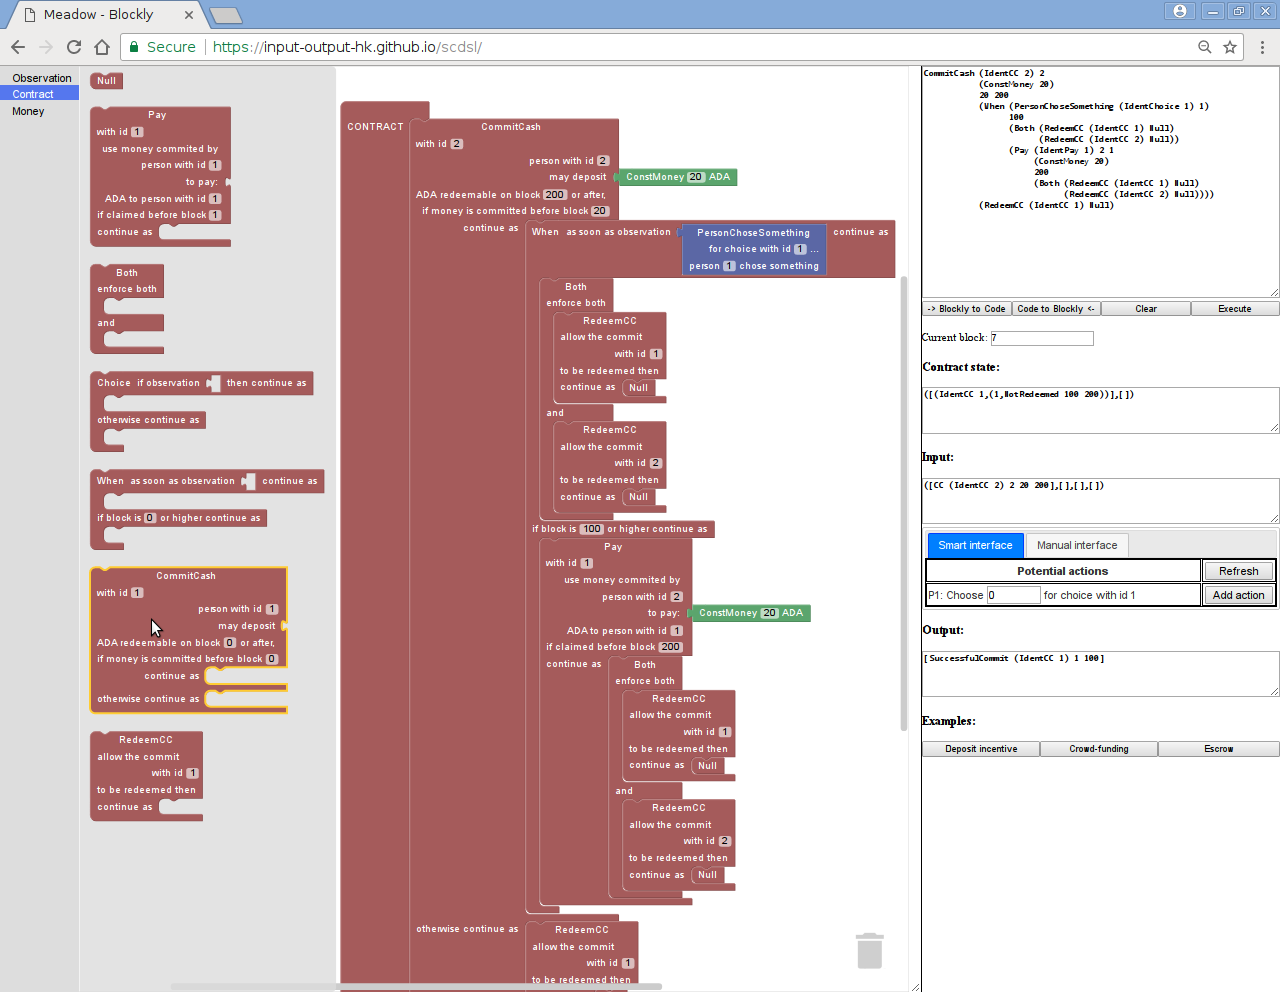
\includegraphics[width=1.1\textwidth]{pix/screenshot1}
\par\end{centering}
\caption{\label{fig:full-screenshot-demo}The Meadow tool
simulating the ``deposit incentive'' contract.}
\vspace*{-6mm}
\end{figure}

%\begin{figure}
%\centering{}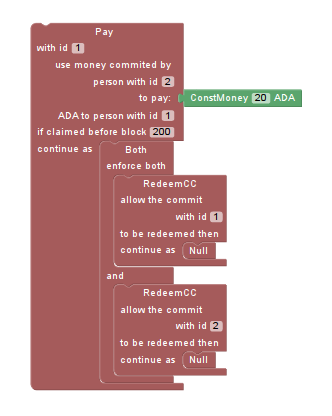
\includegraphics[scale=0.5]{pix/detail1}\caption{\label{fig:detail-of-block}Detail of five interlocked 
%blocks.}
%\end{figure}

The execution of complete contracts can be simulated block by block
by using the panel on the right (see Figure~\ref{fig:detail-of-interface}),
which includes text fields to view and edit the current block number,
the state of the contract, the current inputs, and the outputs from
last block.

\begin{figure}[t]
\centering{}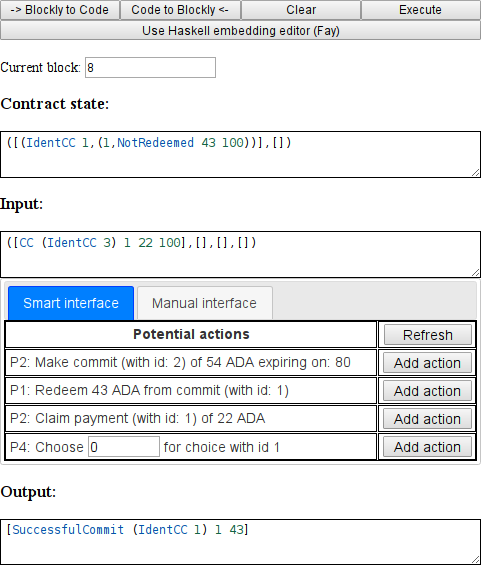
\includegraphics[scale=0.52]{pix/detail}\caption{\label{fig:detail-of-interface}Detail of the interface for 
contract
execution simulation.}
\vspace*{-5mm}
\end{figure}

Additionally, to facilitate the introduction of inputs, Meadow provides
two different interfaces:
\begin{itemize}
\item The manual interface, provides a template for each of the four possible types of input:
commits, redeems, payment claims, and choices.
\item The smart interface (shown in Figure~\ref{fig:detail-of-interface}),
calculates the possible operations that would make sense given the
current inputs, state of the contract, block number, and remaining
contract; and it provides them in a table with most of the parameters
already filled in.
\end{itemize}
%\begin{figure}
%\begin{centering}
%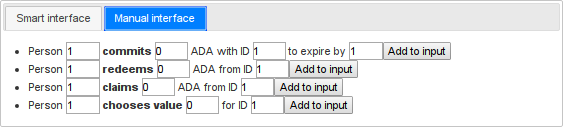
\includegraphics[scale=0.5]{pix/detail3}
%\par\end{centering}
%\caption{\label{fig:detail-of-manual-interface}Detail of the manual interface.}
%\end{figure}
%
%\begin{figure}
%\centering{}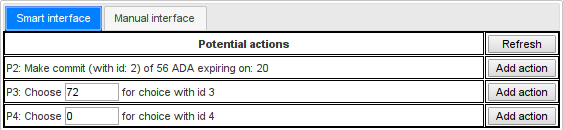
\includegraphics[scale=0.5]{pix/detail4}\caption{\label{fig:detail-of-smart-interface}Detail of the smart 
%interface.}
%\end{figure}

The smart interface is usually more convenient to use than the manual
interface since the later provides between 3 and 4 fields for each
operation whereas the former ``guesses'' the possible intentions
of the user and usually can input new operations with a single click 
(except for choices, which still may require the user to input a number).

%\begin{figure}
%\begin{centering}
%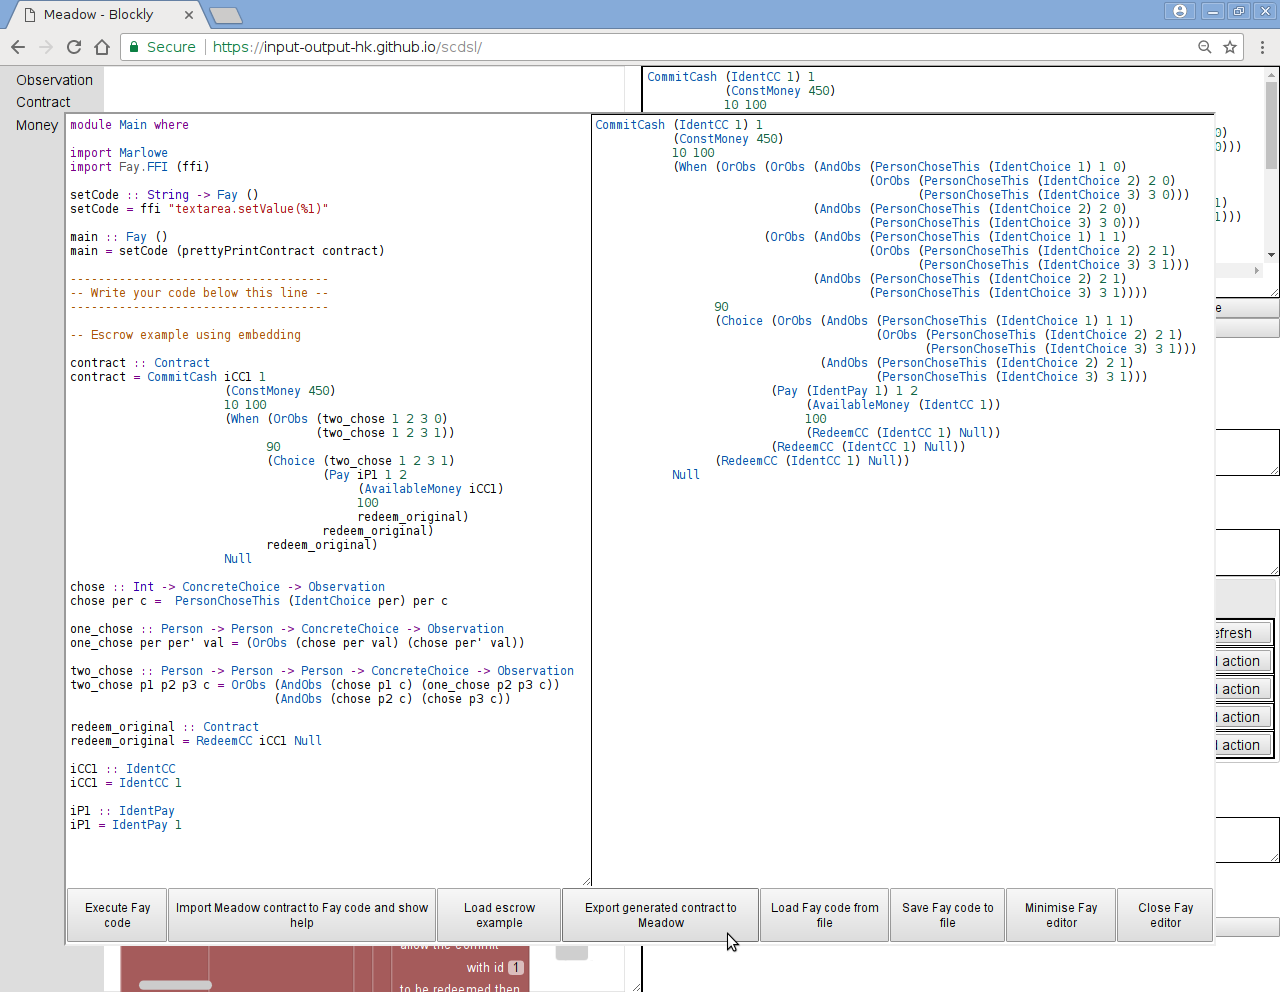
\includegraphics[width=1\textwidth]{pix/embedded.png}
%\par\end{centering}
%\caption{\label{fig:embedded-demo}Screenshot of Meadow's embedded Fay editor.}
%\end{figure}

In the next section, we re-examine the model and the Marlowe language, looking at possible extensions, alternative 
design decisions and ways in which we can formally analyse Marlowe contracts.




\section{Design and Implementation}
\label{section:towards-implementation}

Marlowe is defined by its executable semantics, but to be deployed on blockchain it will have to be implemented on an 
existing distributed infrastructure.  We intend to deploy it on IOHK's Cardano infrastructure, but it can be implemented 
in other systems too, as we explain now.

\subsection{Design Rationale}
\label{sec:abstraction}
\label{sec:design-rationale}

Marlowe abstracts away from a number of concrete details of how blockchains operate. In particular, it is agnostic 
between UTxO-based systems, such as Bitcoin and Cardano SL, and account-based models such as Ethereum; it can be 
implemented on ``push'' or ``pull''-based systems, and can be executed on or off-chain. 

\paragraph{UTxO and accounts}

Transactions on Bitcoin are made by spending the (as yet) unspent outputs of 
previous transactions (`unspent transaction outputs' or UTxOs). The chain need not maintain any state, such as the 
current value owned by any particular participant: such \emph{account} information is implicit and external to the 
Bitcoin blockchain. On the other hand, the Ethereum model explicitly keeps track of account values, and  this 
information needs to be kept on chain. Of the two, the UTxO model is simpler and requires less support from the 
implementation of the chain itself.

\paragraph{Interaction modality}

Contracts can be conceived of as acting in two ways. In a \emph{push} model, contracts are seen to make things happen. 
In the case of blockchain, this would include making payments or transactions take place. 
Alternatively, in a \emph{pull} model, contracts enable certain things, such as transactions,  to happen but the 
transactions need to be effected by an external actor. The pull model makes fewer demands on the blockchain 
implementation than the push model.

\paragraph{Layered design and sidechains}

Some chains have a layered design, in particular Cardano~\cite{cardano}. The Cardano Settlement Layer (SL) is to 
support settlement of transactions but nothing more complicated, whereas the Computation Layer (or CL) supports more 
powerful general computations over the chain. Moreover, the Cardano roadmap~\cite{cardano-rationale} envisages the 
possibility of computation taking place, in part at least, on a sidechain rather than on the main chain itself, which 
may support only the SL. Other off-chain approaches include the Lightning network, overlaid on blockchains (usually 
Bitcoin) and the channels of \ae{}ternity~\cite{aeternity}.



\subsection{Compilation}
\label{sec:compilation}

We have designed Marlowe assuming that each contract would be compiled into
\begin{itemize} 
\item one or more on-chain programs and 
\item a client side program or interface that has a limited number of choices to be made at each point in time 
(including an interface for the observables). 
\end{itemize}
The contracts implemented in the Marlowe language have an implicit interface defined for what would correspond to the 
client side of a distributed application, as shown by the interactive interface. Of course, we probably do not want to 
give a user a programmatic interface but an actual application with user interface. 
%So there is still some work to be done to create interfaces on top of the client side of the contracts.

A contract written in Marlowe could also be potentially
compiled to a smart-contract written in Ethereum. This could be done in two ways: it could be compiled so that a 
smart contract represents a single instance of the Marlowe contract with a fixed set of participants; 
alternatively it would be possible to create a generic contract with an extra ``instantiate'' operation that 
sets up a new Marlowe contract instance with a given set of participants (set of public keys).

\paragraph{Transactions}

In principle, we can directly translate each operation in the model (i.e: cash commitment, payment claim, choice, or
redemption) into a separate transaction in the blockchain. In the Ethereum model this would work in the same 
way that is simulated by Meadow: several operations can be issued in parallel and the blockchain subsystem will 
automatically apply them in some order and integrate them into the next block.

Another approach would be to use a UTxO model with continuations in which a UTxO represents a contract. In this model,
an operation would correspond to a transaction that spends a UTxO and creates (at least) a new UTxO that represents the 
contract after the operation.

Usually, in the UTxO model, it is necessary that a UTxO is in the blockchain in order for another transaction to be 
able to spend it. This could potentially limit the number of operations that can be applied in a single block to one, 
which would make infeasible the approach of using the same UTxO to represent several instances of the same contract 
(since it would not scale).
On the other hand, it would prevent non-determinism and, with it, it would remove the possibility of race-conditions. A 
change to the state of a contract before a transaction (and its corresponding operation) is accepted in the blockchain 
would invalidate the transaction and require the user to issue it again.

Even if we only allow one transaction per block, it would still be possible to combine several transactions off-chain 
and to issue a transaction that contains several operations. However, that would require an offline protocol 
independent from the blockchain and it would require participants to collaborate.

Nevertheless, there already exists in Bitcoin a mechanism that allows the combination of several chained transactions 
within a single block while using the UTxO model, even though it is used to solve a different problem and it is not 
widely spread yet. This is the case of "child pays for parent", which allows the recipient of an unpublished transaction 
to issue another transaction that spends the former, with the aim of including enough fees for both transactions to have 
enough incentive to be included by a miner in a block (in which case both transactions would be included in the same 
block).

The same mechanism could be used for allowing miners to aggregate several transactions that act as a chain in the same 
block. The clients would only need to monitor the transaction pool in order to send transactions that can be chained 
with the existing ones.

\paragraph{Cost}

The Cardano platform has a notion of cost, and Marlowe contracts will potentially incur costs of two kinds: The cost of 
a single transaction execution (e.g.\ a single Plutus validator), and the cost of the whole contract, which may consist 
of many transactions.

Even in Ethereum this distinction is important because single contract execution is limited by gas (and is thus 
finite), whereas the life of the whole contract may be unbounded and consist of an indefinite number of transactions.  
So far we are assuming contracts defined in Marlowe to be finite in both aspects. 
%They could be infinite if we were to 
%define them co-inductively as recursive members of the DSL type.

\paragraph{Recording information on chain}

Inputs and values of observables need to be recorded somehow, and this raises the potential issue about bloating 
the chain with data. In general, it will only be necessary to store a signed hash value of the observable, and this will 
keep data usage bounded; but the full information may still need to be posted in case of dispute.


\paragraph{General computations}

If we have contracts that involve, for example, the oil price then we may need to convert a published price in USD into 
ADA, using a value for the prevailing USD/ADA exchange rate. This will require a computation: in this case, a 
multiplication. If Marlowe is to be stand-alone then we need to extend it with arithmetic and other operations, but 
we expect Marlowe to be embedded in a suitable language that provides these facilities.

%\paragraph{Sidechains and wallets}
%
%The implementation may split contract execution between the main chain and a sidechain (or chains). This will allow 
%links from Marlowe to work on securing multiparty sidechain games/contracts (MPCs).

\ignore{ % begin ignore

\section{Reflection}
\label{section:reflection}

We have given a concrete model and DSL, namely Marlowe version 
1.3\footnote{\url{https://github.com/input-output-hk/scdsl/releases/tag/v1.3}}.
In this section we examine how the model can be extended, how contacts can be analysed, reflect on different design 
decisions that might be made and discuss some aspects of the implementation of Marlowe within a blockchain environment.

\subsection{Potential additions to the model}

The model that we have discussed so far is deliberately kept as compact as possible. However there are a number of 
potential extensions to the model which we introduce here. 

\paragraph{Value commitments}

We have examined a single kind of commitment, namely a commitment of a certain amount of currency. In different 
applications, such as on-chain game playing of games like poker, a commitment to a value will be required. A value 
commitment would include a choice of a play in a game, which would be chosen and concealed from the other players until 
a later point in play, when it can be revealed. The paper~\cite{kumaresan2015use} makes use of this and other 
cryptographic primitives to enforce the rules of poker while maintaining the cards of each player secret.

\paragraph{A monadic DSL}

Haskell is a pure functional programming language, and uses the \haskellinline{Monad} type class to encapsulate
operations that can potentially have a side effect. Many introductions to monads exist \cite{wadler1990comprehending} 
but for the sake of this discussion it is enough to think of a value of type \haskellinline{m a} where \haskellinline{m} 
is a monad as a ``computation that results in something of type \haskellinline{a}''. The \haskellinline{Monad} API 
allows such computations to be assembled, and then, once assembled, they may be run, in general causing some 
side-effects as a part of the computation.

We can make the \haskellinline{Contract} type monadic, so that new, unique identifiers are automatically generated. 
This gives two nice properties. First, they are guaranteed to be unique; secondly they can be generated only in cases 
where a commit has been made successfully (within the required time period). The 
\haskellinline{do} notation supported by monads allows the generated names to be captured by the \haskellinline{bind} 
operation and referred to later in the computation.


\subsection{Potential model analyses}
\label{section:analysis}

Given that we have a language and a semantics for it, we can examine its properties. These might be properties of 
individual runs of a particular contract, of all runs of a given contract, or indeed properties of all the contracts of 
the language. In this section, we look at two particularly obvious questions, but these are not the only ones that we 
might ask.



\paragraph{What are the valid contracts?}

One possible definition is ``those contracts that do not lead to a \haskellinline{FailedPay} action''.
Given the mechanisms for making and using commitments are limited by timeouts, it should be possible to write contracts 
that have this property, perhaps with some assumptions about the value of observables.
Looking at this in a little more detail, we would expect the following points to hold.
\begin{itemize}
\item For a \haskellinline{Pay} contract a sufficient balance not to produce a \haskellinline{FailedPay}.
\item For \haskellinline{Both} we require a sufficient balance for both contracts combined. Need to think here whether 
the two conjuncts should be independent, or whether a commitment in one half can be used in the other.
\item For \haskellinline{Choice} we require a sufficient balance for the maximum of the requirements of the individual 
contracts. 
\item For \haskellinline{When}, need to ``age'' the existing commitments relative to the new starting point of the 
continuation contract.
\item \haskellinline{RedeemCC} should not happen twice in any execution, so as to avoid a
\haskellinline{DuplicateRedeem} action.
\item Are there any constraints on \haskellinline{CommitCash} statements? Not directly, but there need to be sufficient 
funds available to pay if needed, and enough time for the commitments to time out.
\end{itemize}

\paragraph{Do all contracts potentially evaluate to \haskellinline{Null}?}

That is, for each contract do there exist sequences of inputs and observables such that stepping the contract with them 
leads to \haskellinline{Null}? Furthermore, do all sequences of inputs and observables eventually evolve to 
\haskellinline{Null}? Some relevant points include:
\begin{itemize}
\item For \haskellinline{When}, in principle, we would need to be able to make \haskellinline{interpretObs st obs os} 
true. However, since there is  a timeout to \haskellinline{When} then there is no need to impose this condition, as we 
will progress at timeout if not before.
\item As we have put timeouts on to \haskellinline{CommitCash} and \haskellinline{Pay}, the only construct that may not 
reduce to \haskellinline{Null} eventually is \haskellinline{RedeemCC}. \haskellinline{RedeemCC} will still reduce to 
\haskellinline{Null} if the commitment that it refers to has expired (and it will produce a 
\haskellinline{DuplicateRedeem} action), but it will be quiescent forever if the money is never comitted in the first 
place.
\item Other constructs will reduce to \haskellinline{Null} eventually as long as their continuations also reduce to 
\haskellinline{Null} (as is the case of \haskellinline{Both}).
\end{itemize}

\subsection{Questions and alternatives}

The model outlined here raises a number of questions, or suggests a number of alternative choices.

\paragraph{Time}

The model does not take time as an observable, but rather it is defined in terms of \haskellinline{BlockNumber} only. 
We could  use ``slot time'' instead: \emph{``We consider a setting where time is divided into discrete units called 
slots. A ledger, described in more detail below, associates with each time slot (at most) one ledger 
block.''}~\cite{Ouroboros}.

\paragraph{Timelocks}

In systems where time is significant, it is possible to build ``timelocks'' under which it becomes impossible for time 
to progress. Is it possible for block number to depend on progress of computation? We conjecture not, because otherwise 
it would be possible to produce timelocks, under which it would become impossible for time to progress. 

\paragraph{Relative time}

Timeouts are expressed in absolute time: presumably they could be relative (with recording on the blockchain of the 
times at which they are triggered).

\paragraph{Determinism}

The model is deterministic, with all non-determinism being external, and confined to observables. This is surely 
necessary in order to support computation replay, but does it restrict the expressibility of the model?

\paragraph{Causality}

Is there a notion of causality for these contracts? Would we be able to characterise it semantically? Syntactically?

\paragraph{Expiry}

Does a contract expire if a surrounding commitment does? We have not made this a feature of the model.

\paragraph{Premature repayment}

The \haskellinline{RedeemCC} construct is intended for premature repayment of a cash commitment, i.e. before the 
commitment has timed out. Alternatively, it would be possible for the underlying model to repay all committed but 
unspent cash automatically at the end of a contract (but before all commitments have expired), but we might want to do 
the same thing at the end of each ``round'' of  a game, for instance.

\paragraph{Fungibility}

We have modelled cash as fungible: we make payments using the cash commitments in order of expiry time, with those 
expiring earliest being used first. Building a model on UTxO might be a reason for using a different approach.


\paragraph{The \haskellinline{Both} construct}

Does the \haskellinline{Both} constructor potentially produce invalid/misleading contracts, combining a commitment in 
one half with its use in the other? The problem is that this might potentially lead to 
a failed payment. 

\paragraph{Monotonicity}

Some observables have a ``monotonicity'' property: once a choice is made, it is fixed forever; on the other hand, 
something not yet chosen is only so thus far; do we need to reflect this in the observations that we allow?

} % end ignore

\section{Related work}
\label{sec:related}

Blockchains are executed in a replicated form by parties who cannot be guaranteed not to be hostile, either by directly 
trying to change the contents of the chain, or through trying to affect other properties of the chain by indirect means 
(such as swamping honest parties with work). Programming on the blockchain therefore needs to be constrained in some 
ways, since it has to be amenable to replication or verification within a reasonable time if the security and integrity 
of the chain are to be preserved. We look at representatives of the main approaches now; we discuss some of these in 
more detail in an earlier paper~\cite{cryptoeprint:2016:1156}.

\paragraph{Split contracts}
An early work on smart contracts raises the issue that practical contractual situations may well not be amenable to 
complete formalisation, hence giving rise to a \emph{split}~\cite{split-contracts} between an automated part and a 
non-automated part that mediates, for example, real assets. We can foresee that this approach will be needed for Marlowe 
too, if it achieves read-world adoption.

\paragraph{Bitcoin script}

One approach to this is to choose mechanisms such as bitcoin script~\cite{BitcoinWikiScript} which are manifestly 
non-Turing complete. A bitcoin script, written in a Forth-like language, is essentially linear: it can branch, but the 
language contains neither looping constructs nor recursion. It is therefore straightforward not only to see that scripts 
will terminate, but also to give an accurate estimate of the time taken to execute a script. 

\paragraph{Ethereum}

On the other hand, the Ethereum system~\cite{wood2014ethereum} provides a Turing-complete language for the EVM virtual 
machine, and a higher-level programming language, Solidity, that compiles into EVM code. However, EVM and Solidity 
programs are constrained \emph{post hoc} by two mechanisms: program execution must be paid for using `gas' proportional 
to the effort expended, and a set of \emph{ad hoc} limits on program execution, e.g.\ on stack size.

\paragraph{Nxt}

In Nxt~\cite{Nxt}, programmability of the system is provided through a ``fat'' high-level 
API, which is accessible from Nxt clients through a REST interface. The API provides functionality supporting various 
kinds of transactions. The core software itself does not support any form of scripting language; rather, users are 
expected to work with the built in transaction types and transactions that support some 250 primitive operations; these 
can be ``scripted'' in a client (only) using a binding to the API, which is available, for instance, in JavaScript.

\paragraph{Multiple languages}

A common feature of many blockchain platforms is that they provide multiple scripting languages. As we noted earlier, 
Ethereum can be programmed at the EVM level as well as by using the high-level Solidity language. 
Tezos~\cite{tezos-white-paper} supports the stack-based, strongly-typed, functional language Michelson, but also 
provides a high-level language, Liquidity, that compiles into Michelson. Liquidity is also functional and strongly 
typed, but provides more constructs in a more familiar syntax, namely that of a subset of OCaml. 

The \ae{}ternity system~\cite{aeternity} provides multiple languages and VMs~\cite{Stenman-CODE-BEAM}: the functional 
language  Sophia (akin to Reason) and the Functional Typed Warded Virtual Machine (FTWVM) for safe ``system level 
programming'', the language Varna and the HLM for simple contracts, and a (port of) Solidity and the EVM for 
compatibility with Ethereum. In a similar way, Cardano provides support for IELE~\cite{IELE}, a rational reconstruction 
of the EVM, and thus for Solidity too. 

\paragraph{Domain-specific languages} 

A domain-specific language or DSL is a high-level language designed to work in a specific field or domain. The intention 
is that because the users will know about the field, the constructs of the language can be designed to be meaningful to 
them, and also that, because of its nature, the DSL need not include all the features of a general purpose language. 
Removing this clutter and having the remaining operations directly reflect the application area is intended to make the 
language more accessible to domain experts who do not necessarily see themselves as programmers.

Stand-alone DSLs have the advantage of providing appropriate, domain-level error messages when things go wrong, but 
suffer the disadvantage of having to be implemented from scratch. An alternative to this are \emph{embedded} DSLs 
(EDSLs), which provide a ``little language'' for the particular domain embedded within a general-purpose host language. 
This means that parts of the host -- such as arithmetical expressions, or list idioms --  can be used to extend the 
expressibility of the DSL. A notable example of this is the financial contracts language described by Peyton Jones and 
his collaborators~\cite{PeytonJones:2000}, which is embedded in Haskell. Marlowe is similar to the 
DSL in~\cite{PeytonJones:2000} in the use of Haskell embedding, in that the functionality provided is similar, in the use of 
composable combinators, and in the declarative style that allows users to describe what needs to be enforced and not how. 
However the two approaches differ in other aspects like the lack of Marlowe's reliance on the legal system for 
enforcement, its support for multiple party contracts, its explicitness of choices, and its use of a pull model.


%\paragraph{Other approaches}
%
%There are a variety of other approaches to scripting, including business process notations, such as the OMG's BPMN; 
%process calculi such as Rholang; logic rules (in Formal Contract Logic), and finite state machines. More details of 
%these are provided in~\cite{cryptoeprint:2016:1156}.

\paragraph{Findel}

The Findel project~\cite{findel} examines financial contracts on the Ethereum platform, based on the 
seminal~\cite{PeytonJones:2000}, and the authors note that payments need to be bounded; this is made concrete in our 
account by our notion of commitments. They take no account of commitments or timeouts as our approach does, but it 
should be noted that the Ethereum platform is more powerful than the one that we target in this paper.


\section{Conclusions and Future Work}
\label{section:next-steps}

In this paper, we have presented Marlowe, a DSL for financial contracts on blockchains, based on earlier work on 
contracts~\cite{PeytonJones:2000}, together with examples of its use. We have seen that to make this operational on 
blockchain we need to add commitments and timeouts, and to design a semantics that reflects these. As we saw in 
Section~\ref{sec:abstraction}, Marlowe has been designed to make as few demands as possible on the underlying 
blockchain: it can be implemented on UTxO or account-based blockchains, for example.

We have also presented Meadow, that allows users to interact with and simulate the operation of Marlowe contracts, 
contributing to the potential adoptability of the system. We have also described the design rationale for Marlowe, and 
sketched ways in which it can be implemented.

We plan to continue the work with Marlowe in a number of directions. We will continue to develop the core language, for 
example considering the automation of generation of identifiers for commitments and others. We will then implement this 
version of Marlowe in Cardano, compiling from Marlowe contracts to on chain contracts and users' wallets, and deploy it 
in a test network to observe and measure its behaviour in practice.

Building on the operational semantics given here, we will develop analyses of Marlowe contracts -- such as to show that 
contracts cannot generate \haskellinline{FailedPay} actions in certain circumstances. We will also develop  
QuickCheck-style property-based testing~\cite{quickCheck}, and properties developed here can become candidates for fully 
fledged verification in a formalisation of the semantics of Marlowe.

We would like to thank IOHK for supporting us: not only has this led us to work on Marlowe, but we have benefited 
hugely from collaboration with colleagues including Manuel Chakravarty, Duncan Coutts, Bernardo David, Charles 
Hoskinson, Aggelos Kiayias, % Darryl McAdams,
Bruno Woltzenlogel Paleo, Rebecca Valentine and Phil Wadler. We are  very 
grateful to Thomas Arts and colleagues from \ae{}ternity for their convivial discussions on blockchain and contracts in 
G\"oteborg, and to colleagues from the Universities of Kent and Leicester for their comments too.



\bibliographystyle{splncs04}
\bibliography{paper}

\end{document}
